
\begin{figure}[t]
\centering
  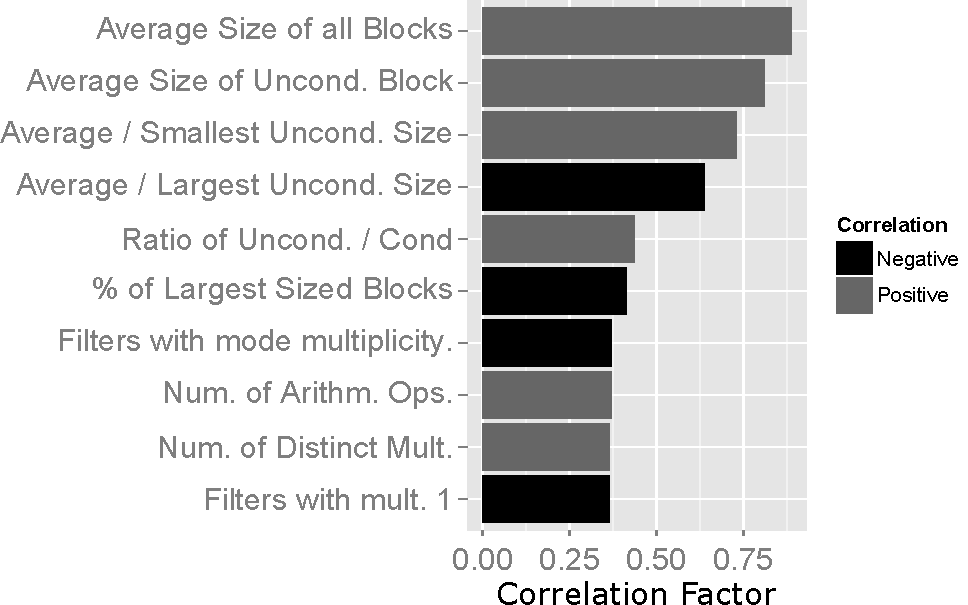
\includegraphics[width=1\textwidth]{streamit-paper/graphics/corrGraph_remix.pdf}
  \caption{The ten highest correlating features with the optimal number of cores.}\label{fig:corrCore}
\end{figure}


\subsection{Gathering Training Data for Core-Composition}
In section~\ref{sec:streamit:dse}, Figure~\ref{fig:threadtrend} shows the performance of each of the 15 benchmarks when partitioning them into threads with and without core-composition.
The figure shows that in both cases, the number of threads is often similar.
Later on in section~\ref{sec:streamit:dse} the use of loop unrolling demonstrates that when blocks are larger more cores can be composed together to improve performance.
With that in mind, in both cases the number of threads does not vary wildly and loop unrolling does not always modify the application to improve the amount of performance that can be extracted via core-composition.
As Figure~\ref{fig:overviewhist} shows that multi-threading outperforms core-composition on its own, it is important to prioritise multithreading.

Therefore predicting core-composition therefore comes after predicting the number of threads.
For this section only the single threaded version of a StreamIt benchmark is used to determine the optimal number of cores.
This allows for the exploration of all possible core-compositions, as partitioning the program into threads can lead to a reduction in the search space.
For example, if the 15 thread versions of the benchmarks were to be used, the could only have a single core allocated per thread when as this is the maximum amount of cores that may be given to each thread rather than it being the optimal solution.

For the exploration of core-composition, only the 15 StreamIt benchmarks are used.
To increase the amount of data available, multiple versions of the benchmarks using different amounts of unrolling are included in the search space.
Four different levels of unrolling are used in this study: 0,4,16 and 64.
To determine the optimal number of cores only the training data that has a performance within 1\% of the best is selected.

\subsection{Analyzing Features}

Figure~\ref{fig:corrCore} shows the highest correlating features with the optimal number of cores.

The ten features can be described as follows
\begin{itemize}
\item Average Size of All Blocks: Average number of operations per block of code.
\vspace{-1em}
\item Average Size of Unconditional Blocks: Average number of operations per blocks that must execute unconditionally.
\vspace{-1em}
\item Average / Smallest Uncondional Size: The ratio between the average size of a block compared to the smallest size of unconditional blocks.
\vspace{-1em}
\item Average / Largest Uncondional Size: The ratio between the average size of a block compared to the largest size of unconditional blocks.
\vspace{-1em}
\item Ratio of Uncoditional Blocks to Conditional Blocks.
\vspace{-1em}
\item Percentage of blocks that have the largest number of operations.
\vspace{-1em}
\item Filters with mode multiplicity: number of filters that have the average mode multiplicity.
\vspace{-1em}
\item Number of arithmetic operations found in the program.
\vspace{-1em}
\item Number of distinct multiplicites found in the program.
\vspace{-1em}
\item Number of filters that have a multiplicity of 1.
\end{itemize}

\begin{figure}[h]
  \center
  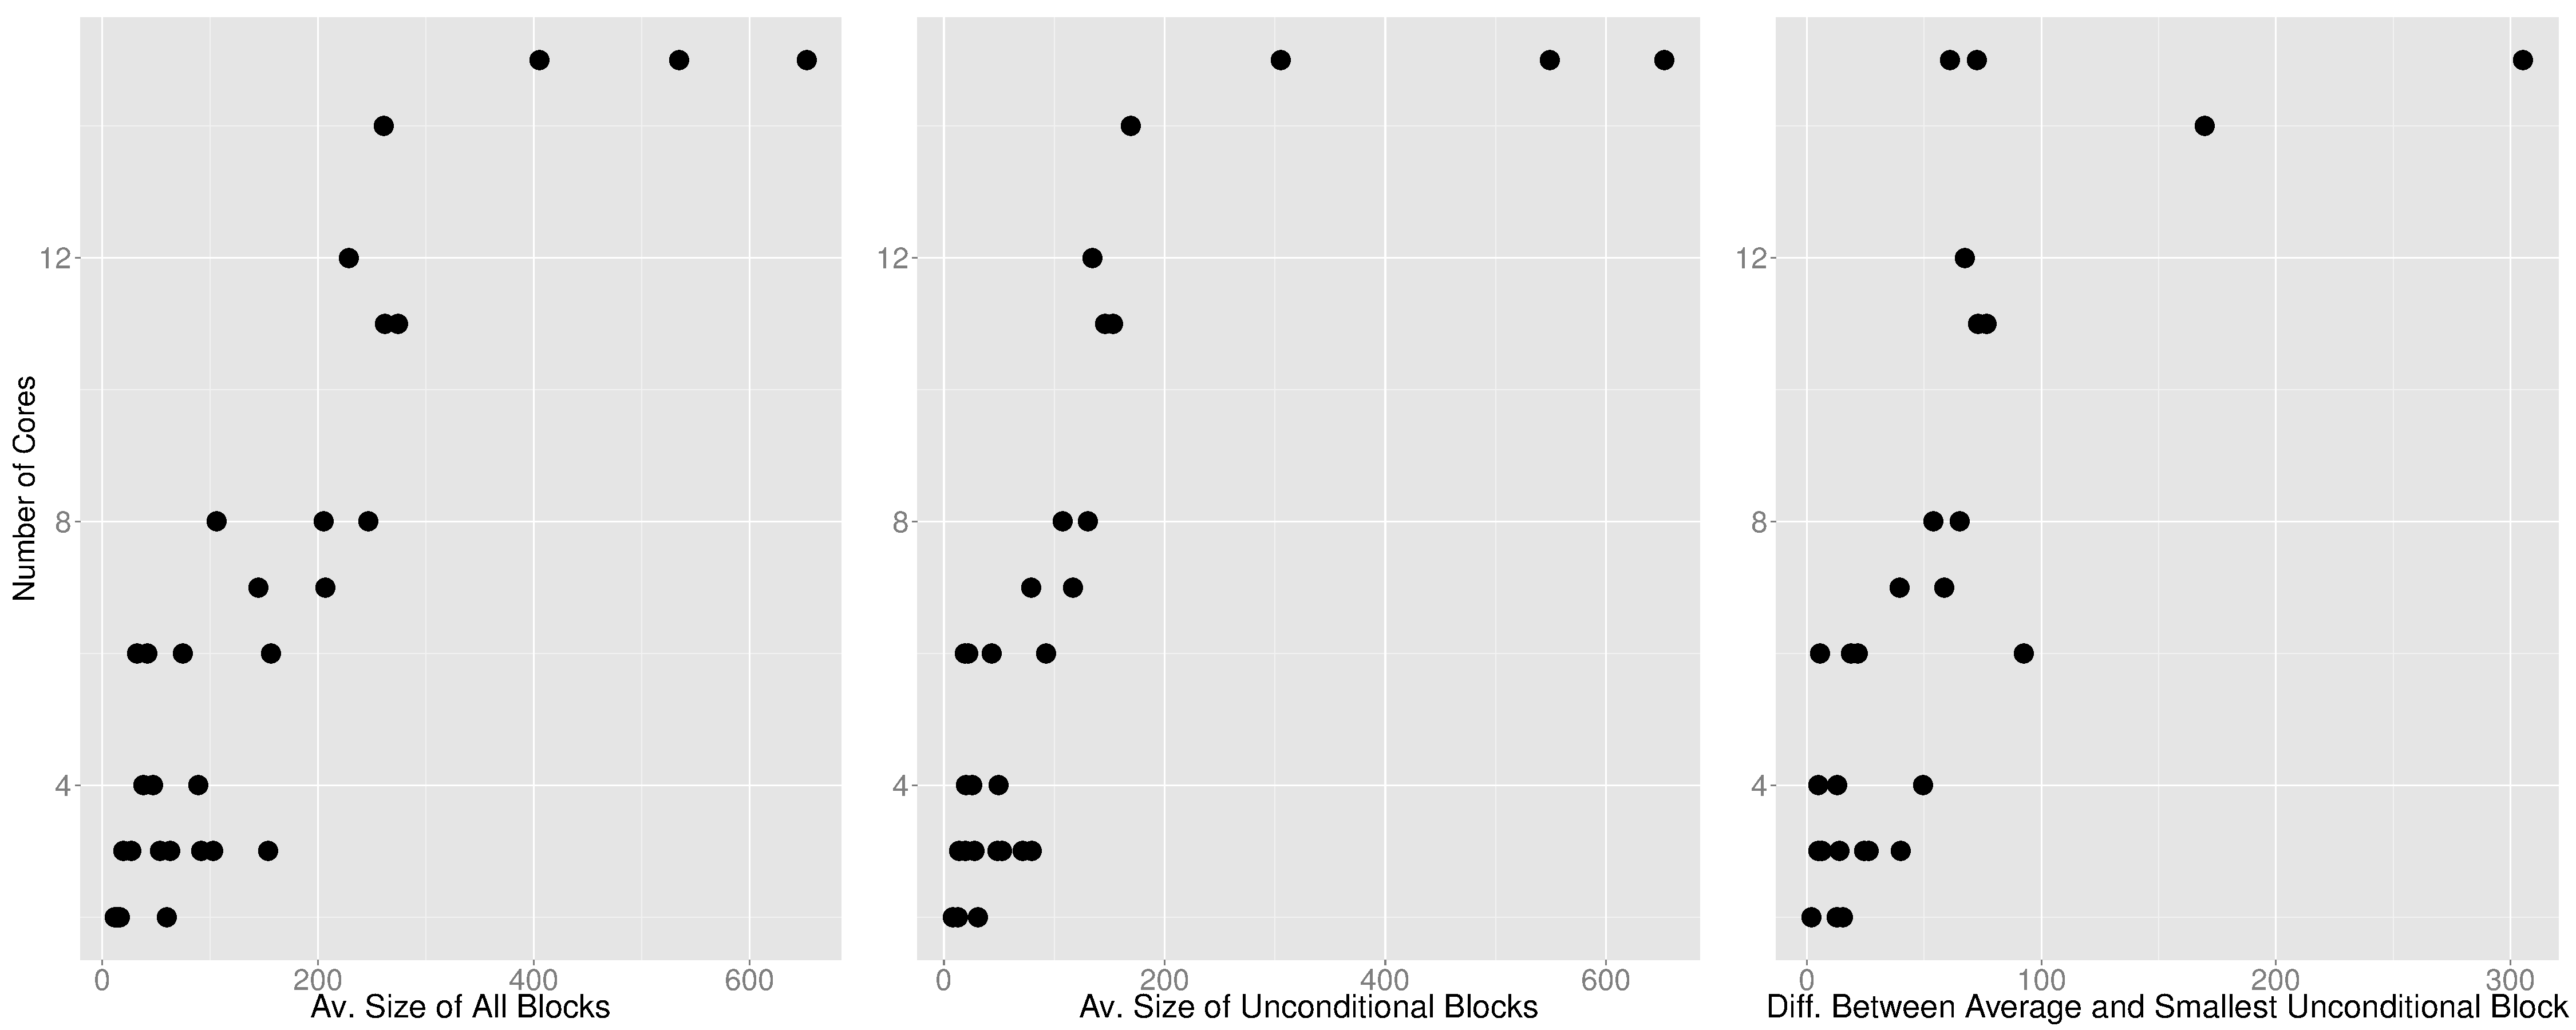
\includegraphics[width=1\textwidth]{streamit-paper/graphics/lineargraphs.pdf}
  \caption{Optimal number of cores in relation to the three highest correlating features. The maximum number of cores plateaus on the right hand side as this is the maximum possible amount.}\label{fig:maxav}
\end{figure}

The features are very different from the ones presented in Figure~\ref{fig:corr} and overall there are features which correlate higher with core-compositions than number of threads.
The highest correlating value has a correlation factor of 0.88.
It is important to note that the concept of an operation here is at the StreamIt level and not the architectural level.
This is due to the fact that the machine learning model will get information from the source-level StreamIt translation.
With that in mind, the number of operations will correlate with number of instructions found at the instruction level.
The second feature is similar to the first but only takes into account blocks that will be executed unconditionally.
Blocks found in loops are excluded for this metric as there is still some form of condition for those blocks to be executed, they are counted as conditional.
The next two feature compare the size of the average size of an unconditional block to the largest and smallest unconditional block.
The fifth feature measures the ratio of the number of unconditional blocks to conditional.

Overall the highest correlating features are not features distinct to StreamIt, such as Pipelines or SplitJoins.
This is due to the fact that, from a single-threaded perspective, SplitJoins and Pipelines are less visible in terms of performance.
This is especially true of SplitJoins as they will not be distributing data amongst different threads and, technically, a single-threaded StreamIt program is a long pipeline structure.
It can thus be infered that the optimal number of cores is independent of the structure of a StreamIt program.
Instead determining the correct core-composition is more dependent on the amount of computation found in each program.

From Figure~\ref{fig:corrCore} the highest correlating features fit naturally under the assumptions that higher core compositions will perform better with larger blocks of operations and thus blocks of instructions.
This is due to the fact that large blocks reduce the amount of branches predictions required to populate all the cores with EDGE blocks which, in turn, reduces the latency of fetching blocks for all cores.
The necessity to correctly predict blocks to ensure that all cores are fully utilised explains why a higher number of unconditionally executed blocks compared to conditional blocks correlates positively with large core compositions.
This is once again due to reducing strain on branch prediction for higher core compositions.
The importance of size is also apparent as the difference between the largest block size and the average block size negatively correlates with core-composition.
StreamIt programs tend to not have a large quantity of conditional statements, thus the ratio of unconditional and conditional blocks is considered less important than the sizes of blocks.

Other features that are analysed included more fine-grained data such as the types of operations that are found in the blocks of code.
This involved finding ratios of floating point, integer and memory operations.
However, according to the correlation graph in Figure~\ref{fig:corrCore}, the constitution of these blocks of code is not as important as their size or whether they are conditionally executed.

%Added text for thesis
%EDGE architecture's ability to fetch atomic instruction blocks and out-of-order execution encourages the focus on determining how much speculation is extracted from each filter.
%Unfortunately StreamIt programs do not tend to have a large quantity of conditional statements and when they do they tend to be quite small.
%This statement is reinforced by the correlation between the average number of conditional blocks with the optimal number of cores, which is only 0.2, compared to 0.809 for the average size of unconditional blocks.
%Thus there is no focus on using any speculative features from the StreamIt graph.

\subsection{Linear Regression Model}
Given that the optimal number of cores highly correlates with a few features, a linear regressor is a natural choice to predict the best number of threads.
Figures~\ref{fig:maxav} represent how the first three highest correlating values affect the optimal number of cores for a single thread.
This figure is obtained by finding the best number of cores for the single threaded version of each of the StreamIt benchmarks whilst varying the amount of loop unrolling.
It is important to note that the top right corner points will always be flat as only a maximum number of 15 cores can be allocated.
Overall, Figure~\ref{fig:maxav} shows that StreamIt applications with large unconditionally executed blocks will require large compositions.


